\chapter{Introduction}
The neutrino was originally proposed by Pauli in 1930 \cite{pauli} to conserve energy and momentum in the beta decay process,
\begin{equation}
n \rightarrow p + e^- + \bar{\nu}_e,
\end{equation}
for which the electron was earlier shown to have a continuous energy spectrum \cite{chadwick}.
Being a low mass, neutral particle, it was some 25 years before the first detection of neutrino interactions in the Cowan-Reines experiment \cite{cowan-reines} through inverse beta decay,
\begin{equation}
\bar{\nu}_e + p \rightarrow n + e^+.
\end{equation}
Later, the fact that neutrinos come in three flavors was established with the detection of muon neutrinos \cite{danby} and tau neutrinos \cite{donut}, with the earlier discovered particles identified as electron (anti-) neutrinos.

As neutrinos were known to be produced in nuclear reactions, the Homestake experiment \cite{homestake} was proposed in the 1960s to measure the flux of neutrinos produced in the core of the Sun.
This experiment measured significantly lower flux than was expected from theoretical calculations, becoming the so-called ``solar neutrino problem" (SNP).
Many experiments \cite{sage,gallex,gno} confirmed this deficit.
The first hints of a solution to the SNP were found in an an up/down anisotropy in atmospheric muon neutrinos observed by Super-Kamiokande \cite{superk} that would not be expected if muon neutrinos remained muon flavor. 
This flavor change was confirmed for solar neutrinos around the turn of the century when the Sudbury Neutrino Observatory (SNO) experiment \cite{3phase} made a measurement of the solar neutrino flux including all neutrino flavors, finding that the initially electron-flavor solar neutrinos were transformed into muon- or tau-flavor neutrinos before arriving at Earth.
This discovery of flavor change implied a nonzero neutrino mass, and a set of massive neutrino states: superpositions of the mass states form the flavor states described earlier.

Determining the parameters of the mixing matrix that relates the flavor and mass basis has been the forefront of neutrino research for the last 20 years, and has seen great success measuring the rotation between the two bases and the magnitude of mass difference between mass states. 
Currently, the absolute masses of the neutrino states have yet to be determined, with the best constraints coming from cosmology, which still only sets a limit on the sum of the mass states \cite{pdg}.
Further, the origin of neutrino mass, be it Dirac or Majorana, is an open question being explored by the current generation of detectors, such as {\snop} \cite{snop}, CUORE \cite{cuore}, and LEGEND \cite{legend}, by searching for a process called neutrinoless double beta decay (beta decay where the neutrinos, as their own antiparticle annihilate, and do not appear in the final state -- only possible if neutrinos have Majorana mass terms).

In this thesis I describe the experimental efforts to fully characterize the flux of neutrinos from the Sun.
Included in particular are a physics analysis from both SNO and its upgrade {\snop}, along with calibration and R\&D efforts supporting solar neutrino measurements.
The first analysis, described in \Cref{ch:lifetime}, explores the possibility that neutrinos are unstable particles and could decay into more stable states.
There the well understood flux of $^8$B neutrinos, and the established framework of neutrino oscillations, provides a constraint on the lifetime of neutrino mass states.
Using solar neutrino data from SNO and combining with other solar neutrino experiments, a limit is set on the rate of such decay.
The currently operating {\snop} experiment aims to measure the solar neutrino flux at lower energies in its scintillator phase than SNO was able to observe.
To aid in this effort, \Cref{ch:chsrc} describes the design and evaluation of an optical calibration source for {\snop}, which will be crucial for understanding the photon detection efficiency (energy scale) for solar neutrino measurements.
The second physics analysis, in \Cref{ch:es}, uses the initial light water phase data from {\snop} to measure the flux of $^8$B solar neutrinos using the kinematics of the elastic scatter of neutrinos off of electrons in the light water.
Looking toward the future, the \textsc{Theia} \cite{asdc} experiment aims to make precision measurements of the lower energy solar neutrino fluxes, as well as support a broader platform of neutrino physics.
This would allow \textsc{Theia} to probe open questions about the Sun, such as the concentration of elements heavier than helium in the core, which affects the relative fluxes of different types of solar neutrinos. 
To achieve such a goal, \textsc{Theia} requires a next-generation target material that combines the positive aspects of experiments like SNO and {\snop}. 
In \Cref{ch:wbls} a benchtop experiment to evaluate the optical properties of such a target material is described.
To aid in understanding these topics, the remainder of this chapter is devoted to the theory of neutrinos and particulars of solar neutrinos, while \Cref{ch:detectors} discusses the steps necessary to detect and analyze solar neutrino fluxes.
But first, the theory.

\section{Standard Model Neutrinos}
\label{sec:stdmodel}

The Standard Model of particle physics aims to describe all observed particle phenomenon in a self consistent theory within the framework of Quantum Field Theory.
Notably this theory describes only three of the four fundamental forces -- the strong, weak, and electromagnetic -- leaving gravity for some grander and as yet undetermined theory. 
Allowing for that notable caveat, the Standard Model has been very successful in its description of nature, except in the neutrino sector where the baseline theory predicts massless neutrinos and no flavor change.
One can, however, augment the Standard Model to include neutrino mass and, from that, flavor change follows naturally.

The theory includes three massless vector bosons roughly corresponding to the three fundamental forces, $g^a$, $W^b$, and $B$, where $a=1..8$ and $b=1..3$.
$g^a$ represents the eight colors of gluons, which mediate the strong force.
Linear combinations of $W^b$ and $B$ are responsible for the weak nuclear force and electromagnetic force, whose bosons are typically written as $Z_0$, $W^{\pm}$, and $\gamma$.

Matter is included in the theory as left- and right-handed fermion fields organized into three increasingly massive generations.
Each generation contains two quarks fields, which can be any of three colors, a charged lepton, and a neutral lepton.
In the first generation, these correspond to the up and down quark, the electron, and the electron neutrino. 
These generations are commonly called flavors, which take their names from the charged fermions.

A fourth boson, the spin-0 Higgs, which was recently observed in 2012 \cite{higgs}, is responsible for the observed mass of these fermions through electroweak symmetry breaking.
This mechanism requires coupling between the left and right-handed fields for each fermion.
Notably, only left-handed neutrinos (right-handed anti-neutrinos) have ever been observed, so initial formulations of the Standard Model did not include right-handed neutrino fields.
This led to a prediction that neutrinos are massless particles, which has now been demonstrated false.

To include neutrino mass in the standard model, one must include right-handed neutrinos.
This results in both a Dirac mass term for the neutrino -- as with the other fermions -- and a Majorana mass term.
The search for Majorana mass of neutrinos is actively being investigated by the current generation of neutrino experiments, however, solar neutrino experiments are insensitive to the origin of neutrino mass, so I will only consider the Dirac case, which takes the form
\begin{equation}
\mathscr{L_D} = m_{ij} \bar{\nu}_{Ri} \nu_{Li} 
\end{equation}
where $m_{ij}$ is the neutrino mass matrix, and $\bar{\nu}_{Ri}$, $\nu_{Li}$ represent the right- and left-handed neutrino fields.
If flavor change is disallowed, this matrix must be diagonal.
With flavor change demonstrated, however, this matrix can take any form.
The mass matrix $m_{ij}$ may be diagonalized by some matrix $U$ to find superpositions of neutrino flavor states with definite mass.
This matrix $U$ is known as the Pontecorvo-Maki-Nakagawa-Sakata (PMNS) matrix.

Many of the degrees of freedom in the PMNS matrix are not observable, and it can be parameterized by three ``mixing angles" $\theta_{12}$, $\theta_{13}$, and $\theta_{23}$, and a complex phase $\delta$.
Typically this is done as follows:
\begin{equation}
U = 
\left(
\begin{array}{ccc}
1 & 0        & 0\\
0 & c_{23}   & s_{23}\\
0 & -s_{23}  & c_{23}\\
\end{array}
\right)
\left(
\begin{array}{ccc}
c_{13}              & 0  & s_{13}e^{-i\delta} \\
0                   & 1  & 0                  \\
-s_{13}e^{-i\delta} & 0  & c_{13}             \\
\end{array}
\right)
\left(
\begin{array}{ccc}
c_{12}  & s_{12} & 0 \\
-s_{12} & c_{12} & 0 \\
0       & 0      & 1 \\
\end{array}
\right),
\end{equation}
where $s_{ij} = \sin{\theta_{ij}}$ and $c_{ij} = \cos{\theta_{ij}}$.


\section{Neutrino Oscillation}
\label{ch:theory}

Neutrinos are produced and interact in the flavor basis, with $\ket{\nu_{\alpha}}$ where $\alpha = {e,\mu,\tau}$, however, these are not eigenstates of the vacuum Hamiltonian, whose eigenstates (the eigenstates with definite mass) are denoted as $\ket{\nu_i}$ where $i = {1,2,3}$. 
The flavor basis is related to the mass basis by the PMNS matrix $U_{\alpha i}$ as follows:
\begin{equation}
\ket{\nu_{\alpha}} = \sum_i U^*_{\alpha i} \ket{\nu_i}.
\end{equation}
The free evolution of these states is most easily represented in the mass basis, as these are eigenstates of the Hamiltonian:
\begin{equation}
\bra{\nu_i}H_{0}\ket{\nu_j} = \frac{1}{2E}\begin{bmatrix}
m_1^2 & 0 & 0 \\
0 & m_2^2 & 0 \\
0 & 0 & m_3^2
\end{bmatrix}.
\end{equation}
The survival probability for flavor state $\ket{\nu_\alpha}$ to be detected as flavor state $\ket{\nu_\beta}$ at some later time after free evolution for a distance L is therefore
\begin{equation}
P_{\alpha\beta} = \left|\braket{\nu_\beta(t)}{\nu_\alpha}\right|^2 = \left|\sum_i U^*_{\alpha i} U^{}_{\beta i} e^{- i m_i^2 L/(2E)} \right|^2.
\end{equation}

\section{Solar Neutrinos}

The Sun is powered by thermonuclear reactions that fuse light nuclei into heavier nuclei, releasing energy.
Much of this energy is in the form of electromagnetic radiation, or energetic charged particles, which thermalizes and is radiated away long after the initial reaction.
However, energetic neutrinos produced in these reactions escape quickly and relatively unhindered, making solar neutrinos an excellent probe of the internal dynamics of the Sun.
The following sections discuss the specific processes resulting in solar neutrinos, how the fluxes of solar neutrinos are predicted, and what other considerations must be taken into account to understand the solar neutrino fluxes at Earth.

\subsection{Fusion Reactions}

The primary reaction in the Sun is the proton-proton ($pp$) reaction,
\begin{equation}
p+p \rightarrow ^2\mathrm{H}+e^++\nu_e,
\end{equation}
which produces the most neutrinos, with a flux of roughly $10^{10}$~cm$^{-2}$s$^{-1}$, but has the lowest energy, making $pp$ neutrinos quite hard to detect.
The $^2$He from this reaction is involved in further reactions in the proton-proton chain, resulting in other neutrino fluxes.
Notable among these is the $^8$B reaction, which produces neutrinos that are both high energy, around 10~MeV, and relatively high flux, at roughly $10^6$~cm$^{-2}$s$^{-1}$, making them an ideal candidate for detection in water Cherenkov detectors.
$hep$ neutrinos are higher energy, but the much lower flux of roughly $10^4$~cm$^{-2}$s$^{-1}$ makes the already rare neutrino interactions much harder to identify on top of backgrounds.
Beyond the proton-proton chain, there is also the so called CNO process, involving carbon, oxygen, and nitrogen nuclei. 
Neutrinos produced from the CNO process have energies and fluxes between $pp$ and $^8$B neutrinos.
\Cref{neutrino_spectra} shows the energy spectra and total flux of all known solar neutrinos, where the fluxes represent theoretical predictions.

\begin{figure}
\centering
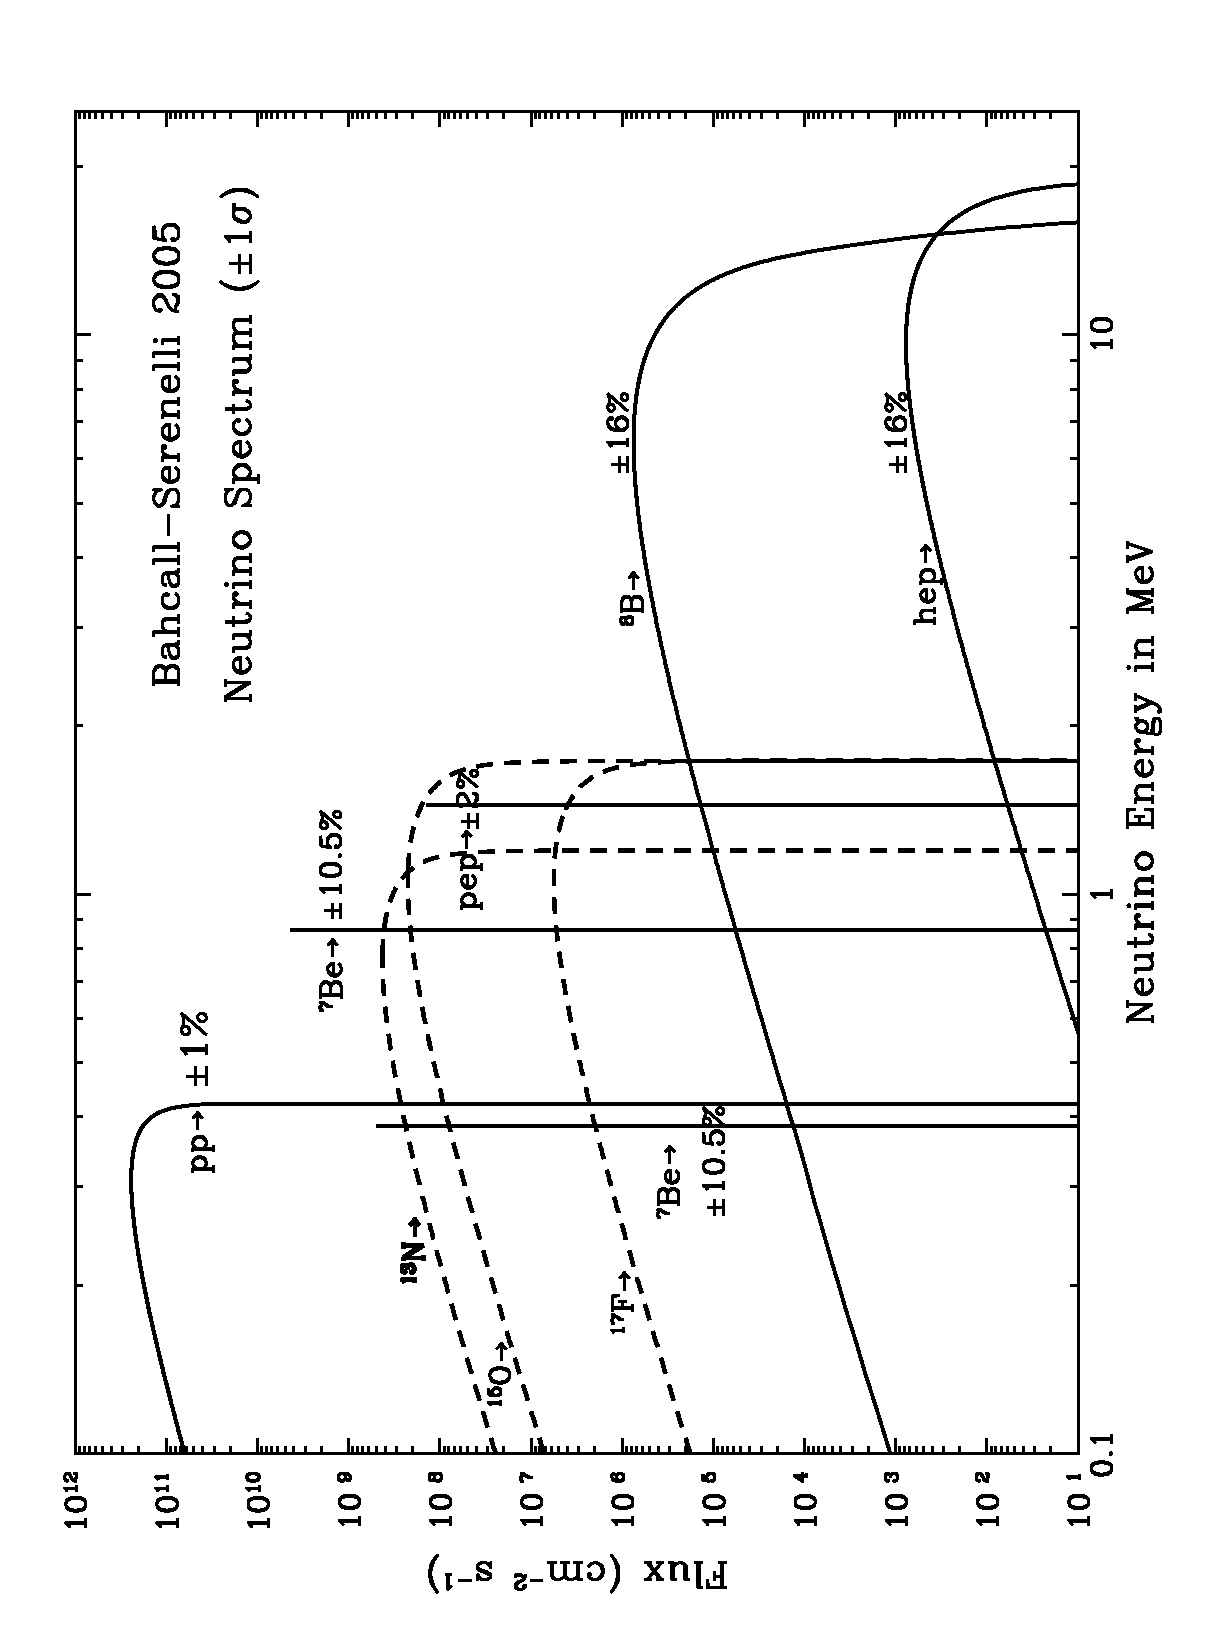
\includegraphics[angle=-90,origin=c,width=0.8\columnwidth]{bachall_bs05op}
\caption{\label{neutrino_spectra}Shown here are the fluxes and spectra of solar neutrinos as calculated in \cite{bs05op}.
    Solid lines show the proton-proton chain neutrinos, while dashed lines show the CNO cycle neutrinos.}
\end{figure}

\subsection{Standard Solar Models}

The fluxes shown in \Cref{neutrino_spectra} are from a theoretical calculation of the equilibrium state of the Sun known as a Standard Solar Model (SSM).
These calculations use hydrodynamic equations of state, contemporary solar observations, and estimations of the primordial composition of the solar system to infer the properties of the solar core.
These properties, such as temperature, density, and isotope content, directly control the rates of the various fusion reactions, and therefore predict the fluxes of solar neutrinos.
These rates depend strongly on predictions for nuclear cross sections at densities and temperatures consistent with the solar core, and uncertainties here drive the uncertainties in the neutrino fluxes.

\subsection{The MSW Effect}

The MSW~\cite{wolfenstein,mikheyev} effect proposes that the coherent forward scattering of electron flavor neutrinos off of electrons in a material adds a potential energy, $V_e$, to electron flavor neutrinos, which depends on the local electron density, $n_e$:
\begin{equation}
V_e = \sqrt{2} G_F n_e.
\end{equation}
Written in the mass basis the Hamiltonian including this effect, $H_{MSW}$, then takes the form
\begin{equation}
H_{MSW} = H_{0} + U\begin{bmatrix}
V_e & 0 & 0 \\
0 & 0 & 0 \\
0 & 0 & 0
\end{bmatrix}U^\dagger.
\label{eq:msw}
\end{equation}
Notably the evolution of the states in the presence of matter is now much more complicated since the eigenstates now depend on the electron density.

It is useful to introduce the matter mass basis, $\ket{\nu_{mi}(V_e)}$, consisting of eigenstates of the Hamiltonian $H_{MSW}$ at a particular electron potential $V_e$.
Note that if the electron density is zero, $H_{MSW}$ reduces to $H_0$. Therefore, $\ket{\nu_{mi}(0)} \rightarrow \ket{\nu_{i}}$.
In many cases the variation of $V_e$ is slow enough that the evolution is adiabatic, meaning some state $\ket{\nu(t)}$ has a constant probability to be one of the instantaneous matter mass states at a later time. 
\begin{equation}
\left| \braket{\nu_{mi}(V_e(0))}{\nu(0)} \right|^2 = \left| \braket{\nu_{mi}(V_e(t))}{\nu(t)} \right |^2
\end{equation}

The electron density within the sun varies sufficiently slowly for an adiabatic approximation to be made.
Therefore, knowing where in the Sun a neutrino is produced (or more precisely the electron density at the production point), one can calculate the eigenstate composition for as long as the adiabatic condition is satisfied.
Once the neutrino reaches the solar radius, vacuum propagation dominates. 
As vacuum propagation does not change the mass state composition of a state, the neutrinos that arrive at Earth have the same mass state composition as those exiting the Sun.
Due to the large distance between the Earth and the Sun, these mass state fluxes can be assumed to be incoherent once they arrive at Earth, and any regeneration of coherence in the Earth is ignored.
Regeneration of coherence while neutrinos propagate through matter is predicted by the MSW effect, and experiments have searched for this by measuring the asymmetry between neutrino fluxes during the night and day (when the neutrinos propagate through the Earth or not).
To date, this regeneration has not been observed to high significance, but the latest results from Super-Kamiokande show a small asymmetry at a bit over two sigma significance \cite{superkiv}.
Therefore, the arrival probability $\phi_i$ of neutrino mass state $\nu_i$ at Earth due to electron neutrinos produced at an electron potential $V_e$ in the Sun in the presence of the MSW effect can be calculated as
\begin{equation}
\phi_i = \left| \braket{\nu_{m i}(V_e)}{\nu_e} \right|^2.
\label{rawflux}
\end{equation}
The analytic expression for this value is non-trivial and in practice $H_{MSW}$ is numerically diagonalized in the flavor basis to find $\bra{\nu_{m i}(V_e)}$ at a particular $V_e$ value and compute this projection.

Ultimately the MSW effect is the leading order effect responsible for the observed survival probabilities of solar neutrinos.
These expressions give the probability of electron neutrinos from the Sun interacting elsewhere as electron neutrinos, $P_{ee}$, or as another flavor neutrino, $P_{ea}$:
\begin{equation}
\begin{array}{rcl}
P_{ee} & = & \sum_i \phi_i |U_{ie}|^2  \\
P_{ea} & = & \sum_i \phi_i |U_{i\mu}|^2 + \phi_i |U_{i\tau}|^2
\end{array}
\label{msw_survive}
\end{equation}

For $^8$B neutrino energies in particular, the MSW effect is very important with $\phi_1 \approx \phi_3 \approx 0$, and $\phi_2 \approx 1$ meaning this flux is a quite pure sample of $\nu_2$ neutrinos. 
Lower energy solar neutrinos are not so affected, leading to dynamics closer to vacuum with $\ket{\nu_{mi}(V_e)} \approx \ket{\nu_i}$.
\Cref{fig:global_solar} shows all the solar neutrino flux measurements made to date overlaying the MSW survival probability.
With the leading order effects now understood, the door is open for precision measurements of neutrino, and, in particular, solar neutrino interactions.

\begin{figure}
\centering
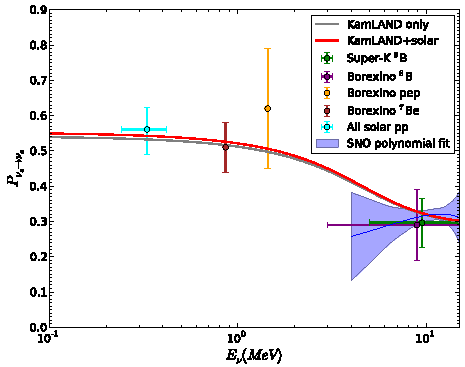
\includegraphics[width=0.8\columnwidth]{all_solar}
\caption{\label{fig:global_solar}Shown here are the measured fluxs of solar neutrinos at various energies by many solar experiments to date as given in \cite{nonstandard_interactions}.}
\end{figure}

\subsection{Open Questions}
The solid lines in \Cref{fig:global_solar} represent the best fit MSW survival probability $P_{ee}$ as determined by combining the measurements of many solar neutrino experiments.
Notably, the error bars on the measurements, from which the best fits are derived, are quite large, leading to considerable uncertainty in the precise shape of $P_{ee}$.
This is of interest because new and interesting physics, such as nonstandard neutrino interactions with matter, would result in distortions to the survival probabilities, which would be measurable by solar neutrino experiments.
Here, ``nonstandard interactions" are any sort of interaction not predicted by the Standard Model that somehow distinguishes between neutrino flavors, and hence influences the propagation of neutrinos in matter.
Much like the MSW effect, the influence from nonstandard interactions would be small, except for the very high densities present in the Sun, making solar neutrinos a viable probe of such effects.
The transition region between vacuum-dominated dynamics below 1~MeV to matter-dominated dynamics above 10~MeV is particularly sensitive to nonstandard interaction, however, this region has not yet been accurately probed by solar neutrino experiments.

To consider a specific possibility, nonstandard forward scattering \cite{nonstandard_forward_scatter} of neutrinos off of fermions is a proposed effect similar to the MSW effect (standard forward scattering of electron neutrinos off of electrons).
Compared to the MSW Hamiltonian given in \Cref{eq:msw}, the Hamiltonian for nonstandard forward scattering allows for all neutrino flavors to couple to matter:
\begin{equation}
H_{NFS} = H_{0} + \sqrt{2} G_F n_e U\begin{bmatrix}
1+\epsilon_{ee} & \epsilon_{e\mu}^* & \epsilon_{e\tau}^* \\
\epsilon_{\mu e} & \epsilon_{\mu\mu} & \epsilon_{\mu\tau}^* \\
\epsilon_{\tau e} & \epsilon_{\tau\mu} & \epsilon_{\tau\tau}
\end{bmatrix}U^\dagger.
\label{eq:nsi}
\end{equation}
where the $\epsilon$ parameters represent the strength of the couplings.
This can be treated in an analogous way to the MSW effect to produce survival probability curves, of which examples can be seen in \Cref{fig:nonstandard}.
Such models cannot be disentangled from the standard MSW effect until higher precision measurements of the survival probability exist in this transition region.

\begin{figure}
\centering
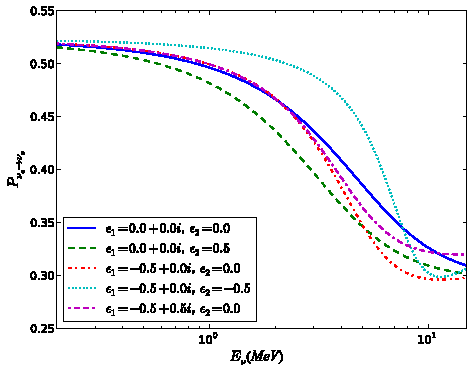
\includegraphics[width=0.8\columnwidth]{nonstandard_interactions}
\caption{\label{fig:nonstandard}Shown here are predictions of the survival probability from nonstandard neutrino forward scattering which cannot be disentangled from the standard MSW effect with existing solar neutrino measurements. The $\epsilon_1$ and $\epsilon_2$ parameter are analogous to the parameters in \Cref{eq:nsi}, but for a two neutrino scenario. Figure from \cite{nonstandard_interactions}.}
\end{figure}

Another possibility, since it is now known that neutrinos are massive particles, is that neutrino mass states could decay to some lighter states.
This can also be treated as a distortion to the survival probabilities, since the signature of neutrino decay is a disappearance (non-detection) of neutrino flux.
An analysis seeking to measure the effect of neutrino decay is discussed further in \Cref{ch:lifetime}, where distortion to the survival probability indicative of neutrino decay is used to set a limit on neutrino lifetime.

Further, the rate of the CNO process in the Sun, which is proportional to the CNO neutrino fluxes, is currently only constrained by analyses done by Borexino.
A high precision measurement of the CNO neutrino flux will provide information about the abundance of elements heavier than helium (``metallicity") in the core of the Sun that are necessary for the CNO process.
At the moment there is tension between standard solar model predictions of metallicity and spectroscopic measurements done of the surface of the Sun, and a better understanding of the CNO neutrino fluxes could resolve some of this tension.
A measurement of the CNO neutrinos is a goal of current and next-generation solar neutrino detectors, however, their low energies and a similarity to the energy spectrum of radioactive contaminates makes this quite difficult.

\clearpage

\chapter{Solar Neutrino Detectors}
\label{ch:detectors}

Neutrinos only interact weakly with normal matter, so the interaction cross sections are quite small, being less than $10^{-40}$~cm$^2$ for energies relevant to solar neutrinos.
Even with expected fluxes of detectable solar neutrinos exceeding $10^6$~cm$^{-2}$s$^{-1}$, the interaction rates are minuscule.
Because of this, neutrino detectors typically rely on large masses of target material to achieve a reasonable interaction rate, with a solar neutrino event a day being quite respectable.
These low rates mean that neutrino detectors must be isolated from cosmic radiation by being constructed deep underground, or lose the neutrino events in the noise.
Even then the materials used to construct the detector must have very low intrinsic radioactivity or suffer the same fate.

\section{Radiochemical Experiments}

The earliest neutrino detectors relied on the transmutation of nuclei by neutrino interactions. 
In the Homestake \cite{homestake} experiment, chlorine nuclei were transformed to argon nuclei via a neutrino capture,
\begin{equation}
\nu_e + ^{37}\mathrm{Cl} \rightarrow ^{37}\mathrm{Ar} + e^-,
\end{equation}
and the created argon was periodically collected its decays counted to estimate the interaction rate in the target volume.
The gallium experiments GNO \cite{gno}, GALLEX \cite{gallex}, and SAGE \cite{sagecombo}, relied on a similar method with gallium:
\begin{equation}
\nu_e + ^{71}\mathrm{Ga} \rightarrow ^{71}\mathrm{Ge} + e^-.
\end{equation}
Notably detectors relying on these radiochemical methods were only sensitive to $\nu_e$ and the solar neutrinos that had oscillated into another flavor were not detected, resulting in the SNP.
Also of note is that these detectors individually provide no information about the neutrinos besides the interaction rate above the minimum energy threshold necessary to transmute the isotope used in the detector. 
Some spectral information can be obtained by looking at results from different isotopes with different minimum energy thresholds, however, event-by-event neutrino energy and direction information is totally lost in the radiochemical detection scheme.

\section{Real-Time Neutrino Detection}

The next generation of neutrino detectors progressed to real-time detection of neutrino interactions.
These were the water Cherenkov detectors, the most recent of which include SNO \cite{3phase} and Super-Kamiokande \cite{superk}, which instrumented a large volume of water with sensitive light detectors that captured flashes of Cherenkov light from energetic particles produced in the neutrino interaction.
Pure water detectors, like Super-Kamiokande, detect neutrinos through the elastic scatter interaction,
\begin{equation}
\nu_e + e^- \rightarrow \nu_e + e^-,
\end{equation}
where the final state electron has a momentum highly correlated with the incident neutrino.

Real-time detectors measure properties about each neutrino interaction as they occur instead of simply counting the number of interactions that happened within a given amount of time.
Analysis of data collected by real-time detectors allows for a statistical determination of the properties of the neutrino flux that produced such interactions.
Real-time detection also allows for different interaction channels to be distinguished, a feature leveraged by the SNO detector, which was instrumental in solving the SNP.

From water Cherenkov detectors, the field has progressed to target media other than water, such as the use of liquid scintillators in Borexino \cite{borexino} and KamLAND \cite{kamland}, which can provide complementary information and lower energy thresholds compared to water.
As this progression is an important theme in this thesis, the following sections go into some details about the merits of each.

\subsection{Cherenkov Radiation}

Ultimately all light from physics interactions detected in water Cherenkov detectors was the result of electrons being scattered with sufficient energy to exceed the local speed of light, commonly called Cherenkov radiation \cite{cherenkov}.
This light is emitted at an angle relative to the direction of the particle track, which depends on the index of refraction of the material.
Because of this, the geometry of the detected hits from Cherenkov radiation can be used to infer the average direction of the electron with resolution of order 10 degrees.
In the cases of ES events, where the electron direction is highly correlated to the primary neutrino direction, this information can be used to disentangle solar neutrino events from backgrounds.
This was leveraged in analyses of SNO data and is a very beneficial feature when dealing with directional sources.

\subsection{Scintillation Light}

As a charged particle moves through a scintillator, electronic energy levels in the scintillator are excited, which can subsequently relax by emitting a visible photon.
In the case of {\labppo} in {\snop}, this results in roughly ten thousand scintillation photons per MeV compared to hundreds of Cherenkov photons.
The much larger number of photons results in much better energy resolution c.f. a water detector, which is very advantageous to analyses that rely heavily on energy reconstruction.

Unlike Cherenkov light, scintillation light is emitted isotropically, since the relaxing of the vibrational state is uncorrelated with the direction of the incident particle.
Further, scintillators are optically less transparent than water (typically) leading to increased scatter (isotropy) in the emitted light.
With much of the Cherenkov light scattered by the scintillator, and the remaining Cherenkov photons buried under two orders of magnitude more scintillation photons, there are very few remaining Cherenkov photons carrying directional information, and those that remain are hard to identify among the scintillation photons.
This leads to the significant downside of being unable to reliably reconstruct direction and, therefore, being unable to disentangle events based on directionality. 
For solar neutrinos this is a significant loss, because typically there is no other class of events correlated with the direction of the sun.
This is applicable both in analyses where solar neutrinos are of interest and should be selected, and also where solar neutrinos would be considered a background and should be rejected.

The final significant difference between Cherenkov and scintillation light is the minimum energy threshold.
Cherenkov light relies on the charged particle being very relativistic (exceeding the local speed of light), meaning that $\alpha$ particles are typically invisible, while betas must exceed 0.7 MeV total energy, to emit any light.
Scintillation, on the other hand, only has the constraint that sufficient energy be deposited to excite vibrational states, typically on the order of eV.
In the case of scintillation, both alphas and betas from radioactive decays are visible, since both can deposit sufficient energy to create scintillation light.
In scintillator detectors, therefore, the maximum rate of the detector electronics are the limiting factor for data acquisition, not the interaction threshold of the medium.
For solar neutrinos, the capability to see lower energy interactions gives access to virtually all types of neutrino fluxes, not just the $^8$B neutrinos accessible by water Cherenkov detectors.
The Borexino \cite{borexino} and KamLAND \cite{kamland} experiments have made excellent solar neutrino measurements with scintillator, and {\snop} plans similar analyses for scintillator phase.

\subsection{Combined Scintillation and Cherenkov Signal}

There are multiple technologies in development with the goal of having simultaneously detectable Cherenkov and scintillation signals, however, for this thesis I will focus on one in particular: water-based liquid scintillators (WbLS).
WbLS mixes a traditional scintillator, {\labppo}, an oil, with water at some configurable ratio that is in large part water.
In principle the fraction of scintillator results in a fraction of total light output from a pure scintillator, so low scintillator fractions will have a comparable number of scintillation photons to Cherenkov photons. 
This leads to enhanced energy resolution compared to only Cherenkov light, while allowing for the possibility of observing Cherenkov geometry in the pattern of detected photons, and thereby obtaining direction information.
At higher scintillation fractions, the relatively fewer Cherenkov photons might be difficult to identify on top of the isotropic scintillation light.
In this case one may leverage the fact that Cherenkov light is very prompt (picoseconds) compared to scintillators ({\labppo} has a short time constant of a few nanoseconds) to potentially identify Cherenkov photons as the most prompt hits.
Finally, being mostly water, WbLS should have longer scattering and attenuation lengths than a pure scintillator, allowing larger volumes to be built before either effect becomes a limiting factor.
This seems to identify WbLS as an ideal material for combining the long attenuation lengths of water with the directionality of Cherenkov light and higher energy resolutions of scintillating materials.
Further discussion of WbLS and a characterization of low scintillator fractions can be found in \Cref{ch:wbls}.

\section{SNO}

\begin{figure}
\centering
    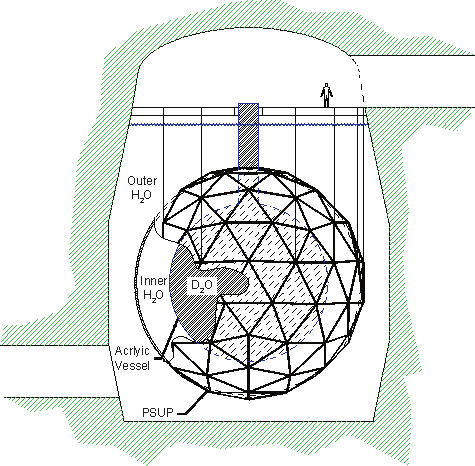
\includegraphics[width=0.8\columnwidth]{sno}
    \caption{\label{fig:sno}The SNO detector as shown in \cite{3phase}.}
\end{figure}

The SNO \cite{sno} detector is located deep underground near Sudbury, Canada in the Creighton mine, an active nickle mine.
This location is one of the deepest laboratories in the world at $2$~km underground, providing a 5800 m.w.e. overburden to shield from cosmic rays.
The detector itself is composed of a 6-m radius acrylic vessel (AV) in the shape of a spherical shell containing 1 kT of heavy water ($^2$H$_2$O or D$_2$O) as the active volume.
Heavy water was chosen because the loosely bound neutron in the deuterons enabled both neutral current and charged current interactions enabling flavor selective measurements of the solar neutrino flux.

\subsection{Neutrino Detection}

As in other water Cherenkov detectors, SNO is sensitive to the elastic scatter (ES) of neutrinos off electrons in the water as shown in \Cref{fig:ES}.
For electron neutrinos, both W and Z bosons can be exchanged.
However, solar neutrinos do not have enough energy to produce heavier leptons, so only Z exchange is possible for non-electron flavor neutrinos.
This means the ES interaction is sensitive to all flavors of neutrino, but with non-electron flavor neutrinos having a lower cross section.
Due to kinematics, the final direction of the scattered electron is highly correlated with the initial direction of the neutrino.
However, the energy is shared between the outgoing neutrino and scattered electron, meaning that the observed electron energy is only loosely correlated with the neutrino energy.
This means that ES interactions give poor spectral information, but very precise direction information.
For solar neutrinos, this means ES electrons will point away from the Sun.

\begin{figure}
\centering
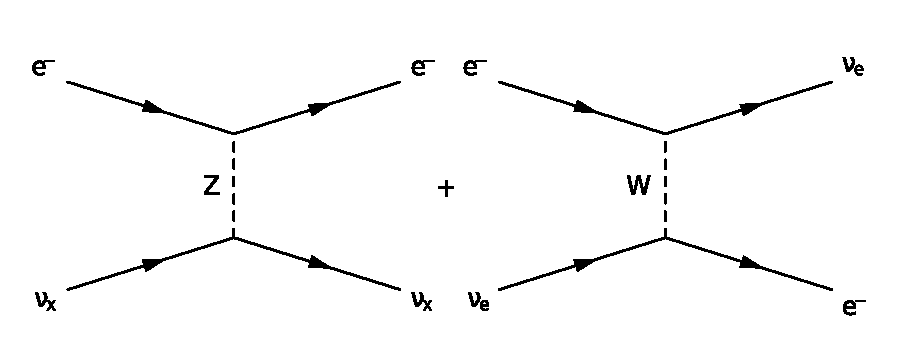
\includegraphics[width=\columnwidth]{feyn_es}
\caption{\label{fig:ES}The Feynman diagrams for elastic scatter (ES) interactions with electrons. 
    Note that all neutrino flavors can exchange a Z boson, but only electron flavor neutrinos can exchange a W boson.}
\end{figure}

The deuterium in the heavy water target used in SNO allows two other types of interaction, each sensitive to different combinations of neutrino flavors.
Most important is the neutral current interaction (NC) due to a neutrino scattering off a quark, as shown in \Cref{fig:NC}.
NC is equally sensitive to all flavor of neutrino, allowing for an oscillation-agnostic measure of the total neutrino flux.
In practice the energy deposited in the quark results in a detectable signal if it exceeds the binding energy of the proton and neutron forming a deuteron.
The liberated neutron will eventually capture on some nuclei, resulting in a cascade of gammas, which can scatter electrons with sufficient energy to produce Cherenkov light.
Due to the detection scheme, information about the energy and direction of the initial neutrino is lost in NC interactions.

\begin{figure}
\centering
    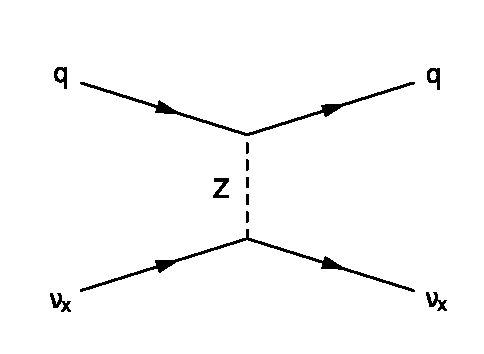
\includegraphics[width=0.6\columnwidth]{feyn_nc}
    \caption{\label{fig:NC}The Feynman diagram for neutral current (NC) interactions with quarks.}
\end{figure}

Neutrinos can undergo a charged current (CC) interaction with quarks in a deuteron, shown in \Cref{fig:CC}.
The CC interaction converts the neutron into a proton, breaking up the deuteron, and producing an energetic electron with an energy correlated to the incident neutrino energy.
In principle any neutrino flavor could participate in a CC interaction, however, solar neutrinos do not have sufficient energy to create heavier leptons.
Muon and tau flavor neutrinos, therefore, cannot exchange a W boson, and do not participate.
The energetic electron then produces Cherenkov light to be detected.
This interaction channel allows for the recovery of spectral information due to the correlation of the electron energy to the neutrino, and provides an exclusive measurement of the electron-neutrino flux. 


The ratio of CC to NC interactions can directly give the average electron neutrino survival probability.
The NC interaction represents a flavor agnostic measurement of the neutrino flux, while the CC interaction is exclusive to electron neutrinos.
This ratio of the two is precisely the definition of $P_{ee}$: the fraction of solar neutrinos detected as electron flavor neutrinos.

\begin{figure}
\centering
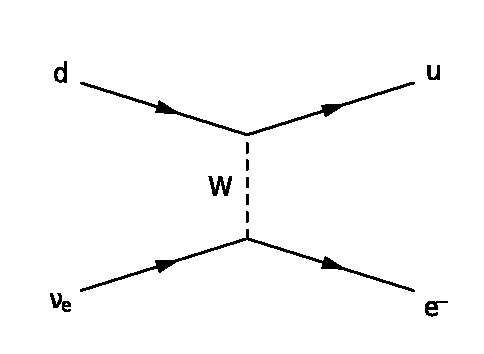
\includegraphics[width=0.6\columnwidth]{feyn_cc}
\caption{\label{fig:CC}The Feynman diagram for charged current (CC) interactions with quarks.}
\end{figure}

\subsection{Experimental Phases}

SNO operated in three distinct phases differing in their neutron detection capabilities, and hence their sensitivity to the NC interaction.
This was achieved by modifying the target material between phases of data taking.
These phases are described in the following sections along with the neutron detection mode in each phase.

\subsubsection{Phase I}

The first phase consisted of a pure D$_2$O target. 
Neutrons produced in the NC interaction primarily captured on other deuterons in the target.
The produced $^3$H then decayed, releasing a 6.26-MeV gamma.
This gamma could either scatter electrons in the target or create energetic electron-positron pairs, either mode being detected by Cherenkov light.

\subsubsection{Phase II}

In the second phase, NaCl was added to the D$_2$O target.
Chlorine has a much greater neutron capture cross section than deuterium, resulting in a significant increase in neutron detection efficiency.
The decay scheme after a neutron capture on Cl is quite complicated, releasing many gammas, and giving these events a more isotropic topology compared to other interactions.
Neutron detection was further enhanced by an increase in total energy released in the gamma cascade to 8.6 MeV.

\subsubsection{Phase III}

Finally, in the third phase, the NaCl was removed from the target, and neutron counting devices (NCDs) were added inside the AV.
These were essentially independent detectors, allowing for an independent measure of the neutron production rate.
A single NCD was a high purity nickel tube containing $^3$He gas, and was instrumented to utilize the $^3$He as a proportional counter for thermal neutrons~\cite{sno_ncd_psa}.
In total, 40 NCDs were added, two of which were modified to contain $^4$He (insensitive to neutrons) to understand instrumental backgrounds.
The NCD data is not directly used in the analysis described in the next chapter, however, it was independently analyzed to constrain the analysis of the PMT data \cite{3phase}.

\subsection{Detector Design}

The target material is contained within a 6-m radius AV.
The AV is surrounded by a 9-m radius steel geodesic structure, containing 9500 inward-facing photomultiplier tubes (PMTs), called the PMT support structure (PSUP).
These PMTs are sensitive to single photons and are intended to capture the Cherenkov radiation from energetic charged particles within the AV.
The entire structure is submerged in a large barrel shaped cavity of light water (H$_2$O) to shield the heavy water in the AV from the natural radioactivity of the mine and other detector materials.
Both the heavy water inside the AV and the light water of the cavity were continually purified to keep intrinsic radioactivity low and cooled to minimize biological growth.

The PMTs used in SNO were 8-inch Hamamatsu R1408 created with low-radioactivity glass. 
These PMTs had a time resolution for detected photons of 1.5~ns, and a peak quantum efficiency of 21.5\% at 440~nm.
Each PMT was outfitted with non-imaging light-concentrating reflectors to increase the effective coverage of light-sensitive elements to 55\%.
To assist in vetoing cosmic rays, 91 additional PMTs were mounted to the PSUP looking outward into the light water of the cavity. 

Whenever a PMT detected a photon, a discriminator would fire on the corresponding voltage fluctuation and register a hit.
This hit started a voltage ramp on a time-to-amplitude converter (TAC) to track the hit time, and integrated the total charge collected by the PMT.
Additionally, the PMT readout electronics would emit two  10-mV square pulses of configurable widths, which are summed across the entire detector and act as a count of coincidentally hit PMTs within each window.
For SNO these windows were set to approximately 20~ns and 100~ns.
The trigger system discriminated the analog sum of each trigger, and, when it crossed a configurable threshold, the trigger system would issue a global trigger (GT) causing all PMTs hit in the last 400~ns to report the value of their TAC (representing the time before the global trigger) and integrated charge (representing the number of detected photons - typically one).
For SNO the discriminator threshold on trigger sums corresponded roughly to 17 hit PMTs.
The hits from each GT are built into a single event for further analysis.

\subsection{Vertex Reconstruction}

To perform an analysis of SNO data it is first necessary to extract physical observables from the PMT hit time information provided by the DAQ.
This is done using pattern recognition algorithms, which take into account the geometry of Cherenkov light to reconstruct the direction, position, and time of each event.
Using that information, along with the total number of hits, other algorithms can estimate the energy deposited in the detector. 
Further quantities can be extracted, such as a measure of the isotropy of the event and the ratio of hits within a prompt time window to all hits, encode additional information about the event that can, for instance, be useful for selecting physics events from instrumental events.
Cherenkov light has a very specific geometry, so good physics events will have a characteristic spatial distribution of detected photons, allowing isotropy to be used to cut instrumental backgrounds.
Similarly Cherenkov light is very prompt, meaning all photons from a physics event are expected to arrive within tens of nanoseconds, and making the ratio of in-time hits a useful metric for identifying candidate physics events. 

\subsection{Calibration}

To understand detector response and characterize the algorithms that perform the vertex reconstruction, sources with known energy spectra or well defined photon emission times that can be deployed at known positions within the detector are critical.
Two sources were critical in this effort:
\begin{description}
\item[\N \cite{sno_n16}] This isotope is produced with a deuterium-tritium neutron generator by captures on $^{16}$O producing $^{17}$O, which quickly decays by emitting a proton to leave \N. This isotope is transported in gas form to a calibration source within the detector where it beta decays into a metastable state of $^{16}$O that relaxes, releasing a 6.13-MeV gamma. The initial beta decay provides a tag signal within the source, and the gamma escapes into the detector where it deposits its energy. This source provides the energy scale calibration for SNO by calibrating its photon detection efficiency. It is also used to evaluate energy and position reconstruction systematics as a function of position within the detector and throughout the operational time of the detector.
\item[Laser Ball \cite{sno_laserball}] A fast dye laser is fiber coupled to an optical diffuser, which work together to produce an isotropic light pulse at a well defined time. This is primarily used to calibrate the time offset of each PMT, and can also be used to measure relative detection efficiencies of the PMTs.
\end{description}
Additional sources were used to provide calibration points at other energies, such as a beta source using \Li \cite{Tagg:2002} with an endpoint at 14~MeV, and a proton fusion source \cite{fusion_source} producing a gamma at 19.8~MeV.
Sources producing the decay chains of $^{238}$U and $^{232}$Th were deployed for low energy calibrations.
Additionally, the heavy water target was at times intentionally spiked with both radon and $^{24}$Na to provide calibrations unbiased by the presence of shielding that is unavoidable in encapsulated sources.
Finally, to characterize the neutron detection efficiency critical for the measurement of the NC interaction, two neutron sources were deployed: $^{252}$Cf and an AmBe source.

The deployed sources were lowered into the detector through the neck via the manipulator system.
This used a central umbilical to provide power or gas-transport to the sources, and additionally used a rope system to accurately position the sources within the detector volume.

\subsection{Previous Results}

As mentioned, SNO was instrumental in demonstrating flavor change of solar neutrinos, and this was possible by using the flavor discrimination of the available interaction channels.
By using the distinct signatures of NC, CC, and ES events, SNO was able to measure the rates of each type of interaction.
These rates could be converted into incident neutrino fluxes, $\Phi_{NC}$, $\Phi_{CC}$, and $\Phi_{ES}$, by unfolding the detector response and interaction cross sections (with assumptions about the spectral shape of $^8$B neutrinos).
Then knowledge of the flavor discrimination of each interaction channel allows constraints on these fluxes to be constraints on the flavor components, $\Phi_e$ for electron flavor and $\Phi_{\mu\tau}$ for muon and tau flavor, of the overall neutrino flux:
\begin{equation}
\begin{split}
\Phi_{NC} &= \Phi_{e} + \Phi_{\mu\tau} \\
\Phi_{CC} &= \Phi_{e} \\
\Phi_{ES} &= \Phi_{e} + \epsilon \Phi_{\mu\tau} \\
\end{split}
\end{equation}
where $\epsilon$ represents the relative interaction cross section for electron and other flavor neutrinos.
Graphically this is shown in \Cref{fig:sno_flavor}, which conclusively demonstrates a non-electron flavor component to the total neutrino flux.

\begin{figure}
\centering
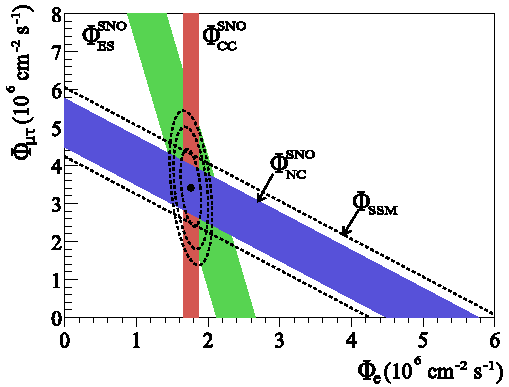
\includegraphics[width=0.8\columnwidth]{sno_flavor}
\caption{\label{fig:sno_flavor} Direct evidence for flavor change in solar neutrinos from SNO taken from \cite{sno_direct}.}
\end{figure}

Later SNO analyses, such as the Low Energy Threshold Analysis (LETA) \cite{leta} of Phases I and II of SNO data, or the extension of this including Phase III data, aptly referred to as the 3-phase analysis \cite{3phase}, were able to fit directly for the survival probability $P_{ee}$ as a function of neutrino energy.
Since neutrino energy is not something SNO observed directly (the ES and NC interactions give little to no spectral information), a method was developed to determine the impact of $P_{ee}$ on observable quantities.
Since $P_{ee}$ can be taken as the fraction of neutrinos that are electron flavor as a function of energy, weighting the $^8$B energy spectrum used to describe $\Phi_e$ properly accounts for the energy dependence of $\nu_e$ survival.
In the same way, the $^8$B energy spectrum for $\Phi_{\mu\tau}$ may be weighted by $1-P_{ee}$ to account for the neutrinos converted to $\nu_\mu$ or $\nu_\tau$.
To making assumptions about the shape of the survival probability, SNO opted to parameterize $P_{ee}$ by a second degree polynomial.
The result of this style of analysis can be seen in the earlier \Cref{fig:global_solar}.
By comparing the fitted survival probability to models of neutrino propagation, most notably the MSW model described earlier, SNO was able to constrain neutrino oscillation parameters.
Building off this style of analysis one is able to probe neutrino physics as a function of neutrino energy and investigate other effects beyond MSW that would influence neutrino propagation.

\section{\texorpdfstring{\snop}{SNO+}}

The SNO experiment finished taking data in the early 2000s, and an upgrade of the detector was planned, which ultimately led to {\snop} \cite{snop}.
The primary goal of {\snop} is a measurement of neutrinoless double beta decay, which, if observed, would shed light on whether the neutrino is its own antiparticle and on the nature of neutrino mass.
Also included in the goals of {\snop}, and of particular relevance to this thesis, is a measurement of lower energy solar neutrino fluxes, particularly the CNO neutrinos, enabled by a switch of target mediums to a scintillating liquid also necessary for neutrinoless double beta decay sensitivity.
To enable this change in targets, some modifications to the experiment were necessary: the detector electronics required upgrades to handle the higher data rate expected with lower energy thresholds, and the AV required the installation of hold-down ropes since scintillator has a lower density than water and would otherwise tend to float in the water shield.
A rendering of the upgraded detector can be seen in \Cref{fig:snop}.
Additionally, the chemical plants to purify and process scintillator, and other supporting hardware, needed to be installed underground, which was no small task.

\begin{figure}
\centering
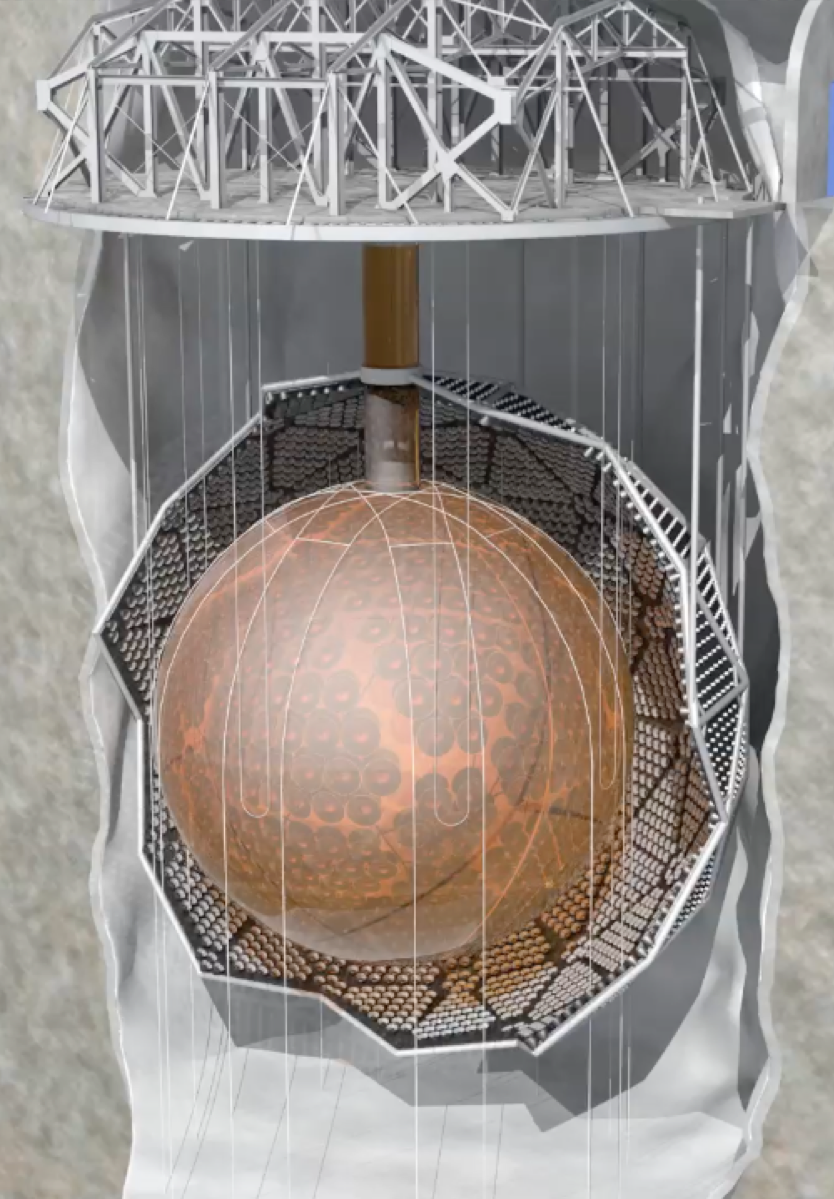
\includegraphics[width=0.5\columnwidth]{snop.png}
\caption{\label{fig:snop}The {\snop} detector. Note the PSUP is only partially rendered to expose the AV.}
\end{figure}

\subsection{Experimental Phases}
Similar to SNO, {\snop} intends to operate in three experimental phases.
The first phase is of primary relevance to this thesis, however, all three are described in the following sections.

\subsubsection{Light Water}
Water phase in {\snop} is intended to calibrate the detector and test the upgraded hardware in a regime similar to SNO, while also generating physics data as a deep underground water Cherenkov detector.
As part of the calibration effort in water phase, \Cref{ch:chsrc} describes an optical calibration source designed for {\snop}, which will be calibrated in water phase and then used to calibrate later phases of the experiment.
Of physics interest in this phase are a search for nucleon decay \cite{nucleon_decay}, potential sensitivity to anti-neutrinos in pure water, and the elastic scatter of solar neutrinos.
Relative to other water Cherenkov detectors, SNO benefits from its deeper location in a reduced muon flux, and hence reduced cosmogenic backgrounds
In terms of solar neutrinos, light water differs from heavy water primarily in the available interaction channels: neither NC nor CC are possible given the lack of targets (deuterons) with sufficiently low interaction thresholds.
The ES interaction is unaffected by this change in targets, since both H$_2$O and D$_2$O have roughly the same electron density.
\Cref{ch:es} goes into detail on measuring the $^8$B solar neutrino flux in {\snop} with the ES channel.
Data taking for this phase began mid 2017 and finished toward the end of 2018.

\subsubsection{Scintillator}

The change to pure scintillator {\labppo} (linear alkylbenzene with a primary flour 2,5-diphenyloxazole at 2~g/L) started at the end of 2018 with the gradual displacement of water inside the AV.
This switch was motivated by a need for enhanced energy resolution for the neutrinoless double beta decay measurement, and similar reasoning comes into play in its applicability to solar neutrinos.
In terms of solar neutrinos, the ES interaction channel is still the only relevant one, however, the observed signals in scintillator phase will be quite different than that of water phase.
In water all information about the interaction was gathered from the Cherenkov light emitted. 
Cherenkov light will still be generated in scintillator, however, in {\labppo} it will be insignificant compared to the light emitted by the relaxing of vibrational states of the scintillating medium itself.
As of the writing of this thesis, scintillator phase is moving forward, but physics data taking is still in the future.

\subsubsection{Tellurium Loaded Scintillator}
As mentioned, the primary goal of {\snop} is to perform a neutrinoless double beta decay measurement using the double beta decay isotope $^{130}$Te.
This will be done by dissolving $^{130}$Te metal in the {\labppo} scintillator, and searching for an excess of events at the endpoint ($Q \approx 2.6$~MeV) of $^{130}$Te decay.
The basic principle behind this measurement is that a double beta decay with neutrinos should follow a double beta decay energy spectrum, where some fraction of the decay energy is not observed due to being carried away by neutrinos, while a neutrinoless decay would deposit the entire decay energy into the the electrons, resulting in a delta function spectrum at the endpoint.
Since the signature of this process is a sharp feature in energy, {\snop} requires the enhanced energy resolution of scintillators, as such a measurement would not be possible with the energy resolution of Cherenkov light.

\subsection{Calibration}

{\snop} makes extensive use of SNO calibration hardware in its calibration effort, however, upgrades of the deployment hardware are planned for scintillator phase to meet the more stringent background requirements of that phase.
For water phase, both the SNO \N and Laser Ball sources were used in the same manner as in SNO.
An upgrade of the SNO Laser Ball is under construction for scintillator phase in {\snop}.
The timing calibration typically by the Laser Ball is intended to be replaced by a fast pulsed LED system called ELLIE, which is fiber coupled to known positions on the PSUP, and does not require deployment of a source into the target volume.
A new calibration source (described in \Cref{ch:chsrc}) intended to replace the \N calibration of photon detection efficiency for scintillator phase was developed.
Finally, new radioactive sources, such as a $^{48}$Sc and $^{57}$Co, are being developed to assist in energy scale calibrations in tellurium loaded phase, while intrinsic radioactivity present in the scintillator provides another means for calibrating energy scale.

\section{\textsc{Theia}}

\textsc{Theia} \cite{asdc_paper} is a proposed large scale (50-100~kT) neutrino detector, which aims to support a diverse platform of neutrino physics. 
Of particular relevance to this thesis is the goal of doing high precision measurements of solar neutrinos \cite{theia_solar}.

\subsection{Conceptual Design}
The detector design is still in the conceptual phase, but lessons learned from {\snop} and other liquid scintillator detectors are being incorporated, and the optical detection scheme remains roughly unchanged except for potential upgrades to technologies similar to PMTs.
The basic plan is two-fold: build a very large detector to maximize interaction rate and enhance fiducial volume shielding, and develop a novel target medium that combines the advantages of Cherenkov and scintillation light.
The former is primarily an engineering and/or funding challenge, while the latter presents an interesting research topic that is explored further in \Cref{ch:wbls}.
The baseline design calls for a right cylinder around 40~m across filled with WbLS and surrounded with fast photo detectors.
The optical clarity of WbLS should allow scaling to these sizes without undue loss of photons to attenuation.

\subsection{Sensitivity to Solar Neutrinos}
With WbLS comes the possibility of simultaneously detecting a Cherenkov and scintillation signal.
The presence of a Cherenkov signal means that the direction reconstruction is again possible, while the scintillation light will enhance the energy resolution relative to water Cherenkov detectors, and allow for detection of events below the Cherenkov threshold.
In particular, simulations suggest \textsc{Theia} would have good sensitivity to the CNO cycle neutrinos \cite{theia_solar}.

Since WbLS for \textsc{Theia} would be primary water, this allows for easy loading of metals into the detector.
Of primary interest are isotopes like $^7$Li, which, like the deuterons in the heavy water in SNO, have low enough binding energies for solar neutrinos to participate in a CC interaction \cite{asdc_paper}.
As the CC interaction has a visible energy much better correlated with the incident neutrino than the ES interaction, loading such an isotope in WbLS in \textsc{Theia} would enable high resolution measurements of the solar neutrino spectra. 



